\chapter{Results} \label{sec:Results}
\section{Identification Problem's Results} \label{sec:Identification Problem's Results}
\subsection{Optimization Results} \label{sec:IdProbRes - Optimization}
Running the 3-layered network with the GPU ``set'' with different learning rates on different seeds (to calculate average performance of each learning rate) for 10000 epochs showed that the model was performing constantly giving lower loss values ($Z_I$ - \Cref{eqn:iden_problem}) with learning rate = $10^{-3}$. 

We observed that higher learning rates ($>10^{-2}$) could only decrease the loss function to a limit, after which the updates in the weights caused the loss function to oscillate and increase. This phenomena is exemplified in \Cref{fig:Test Loss Plots of Different Learning Rates to Find Weights}, which are plots of different models with the same seed but different learning rates. On the other side of $10^{-3}$, lower learning rates took too long to train. Runtime for the model on 10000 epochs was 1232.56 seconds (average over 20 runs = 5 seeds $\times$ 4 learning rates), and models with learning rates less than $10^{-3}$ did not perform better than those with learning rate = $10^{-3}$ on \textit{any} run. Although the decrease in test losses were constant for learning rates less than $10^{-3}$, we feel that they may be computationally expensive and temporally inconvenient to train.
\begin{table}[!htbp]
    \centering
    \caption[Loss Values Calculated for Different Models for Identification Problem]{Loss Values Calculated for Different Models for Identification Problem: For both the 3- and the 4-layered models, learning rate = $10^{-3}$ outperformed other learning rates. Consequently, that learning rate is used in comparison with other models in \Cref{fig:Comparison of Loss Values from Different Models of the Identification Problem}.}
    \label{tab:Loss Values Calculated for Different Models for Identification Problem}
    \begin{tabular}{c | c | c}
        \hline
        \multirow{2}{*}{\textbf{Learning Rate}} & \multicolumn{2}{c}{\textbf{Average Test Loss Values}} \\
        & 3-layered & 4-layered\\
        \hline
        $10^{-2}$ & 0.168 $\pm$ 0.068 & 0.494 $\pm$ 0.083\\
        $10^{-3}$ & \textbf{0.119 $\pm$ 0.016} & \textbf{0.228 $\pm$ 0.048}\\
        $10^{-4}$ & 0.151 $\pm$ 0.040 & 0.237 $\pm$ 0.067\\
        $10^{-5}$ & 0.212 $\pm$ 0.040 & 0.320 $\pm$ 0.067\\
        \hline
    \end{tabular}
\end{table}

\begin{figure}[!htbp]
    \centering
    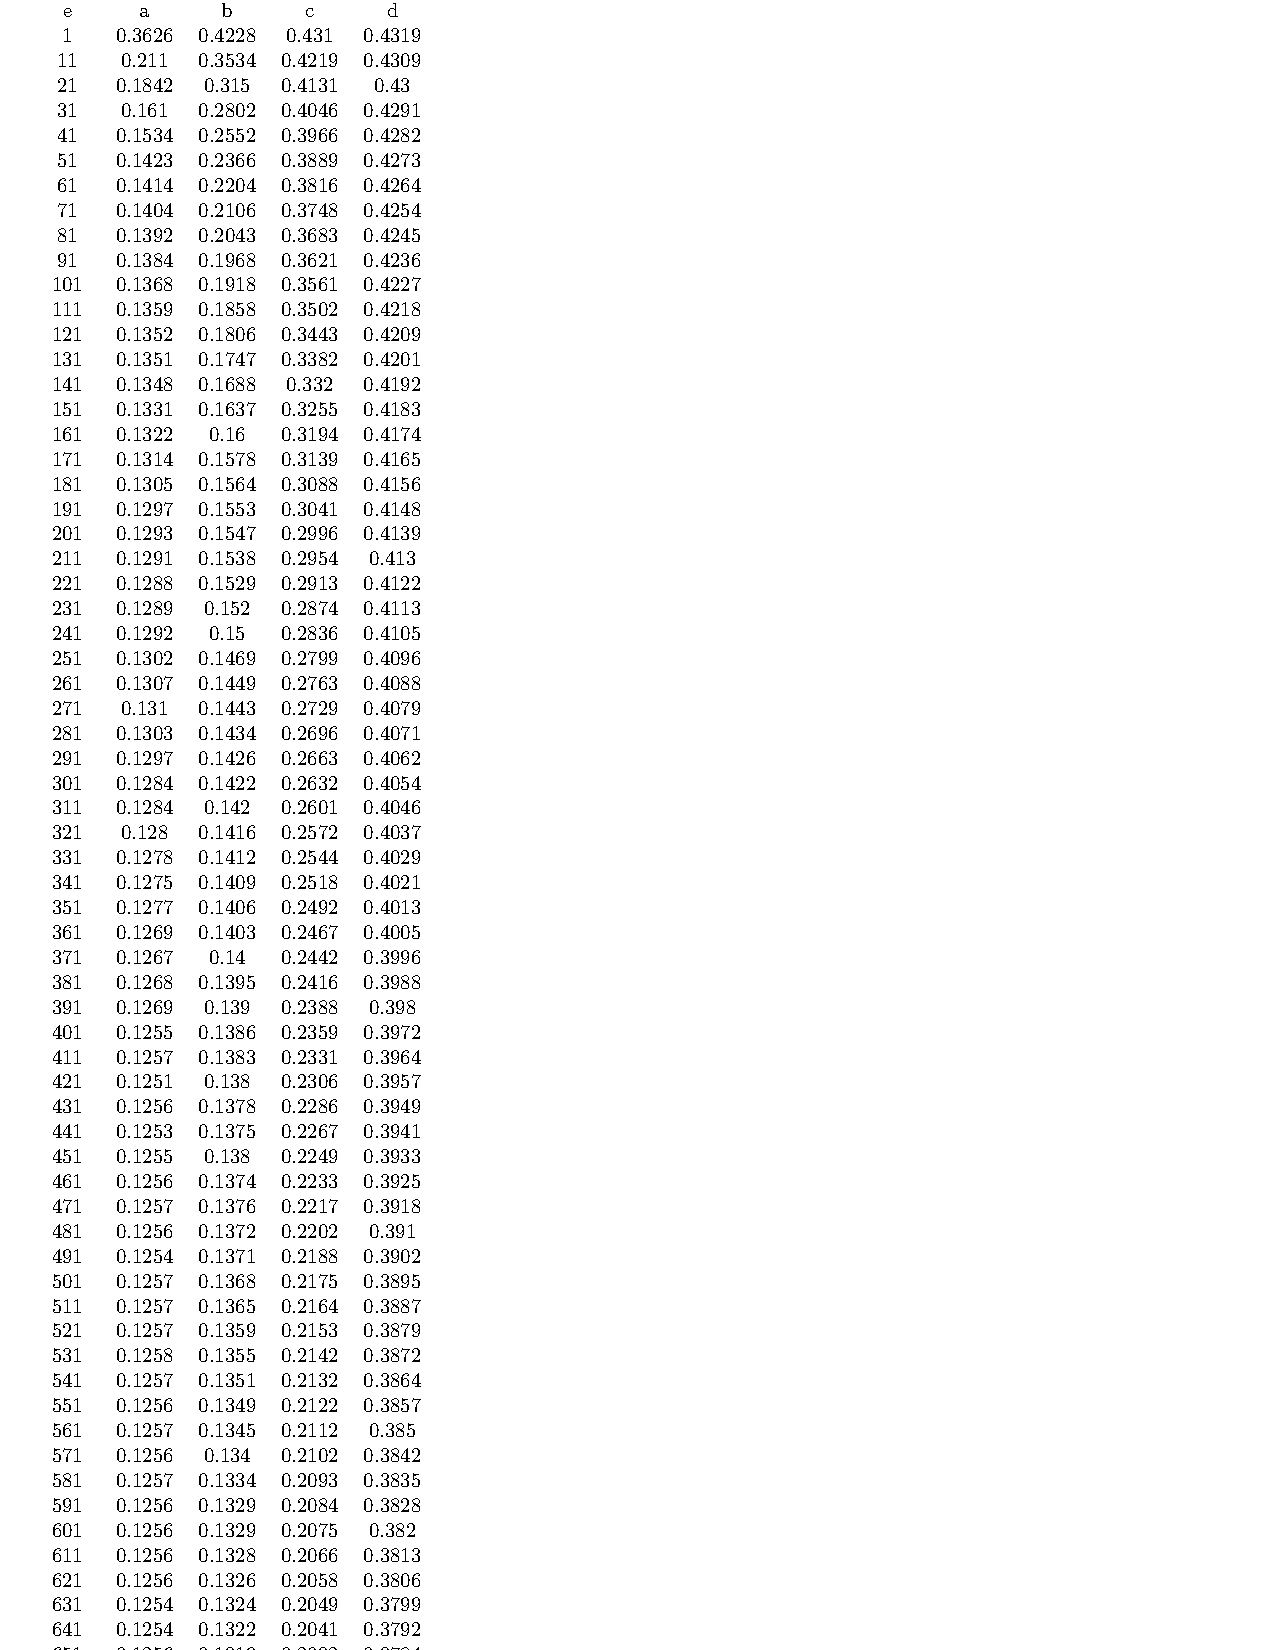
\includegraphics[width=16cm, height=10cm]{test_losses_diff_lr_plot}
    \caption{Test Loss Plots of Different Learning Rates to Find Weights}
    \label{fig:Test Loss Plots of Different Learning Rates to Find Weights}
\end{figure}
\begin{figure}[!htbp]
    \centering
    \begin{minipage}{.48\textwidth}
        \centering
        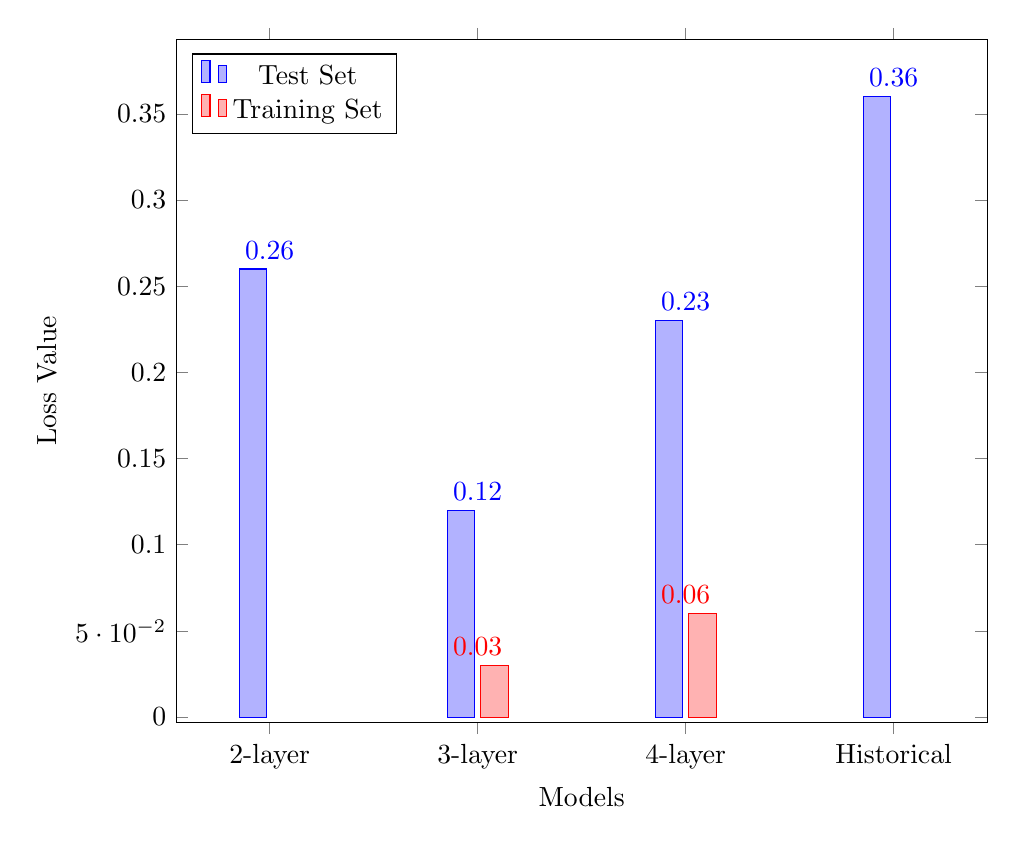
\begin{tikzpicture}
            \begin{axis}[
                ybar,
                width=.98\textwidth,
                enlarge x limits=0.15,
                legend style={at={(0.02,0.98)},
                    anchor=north west,legend columns=1},
                ylabel={Loss Value},
                symbolic x coords={2-layer,3-layer,4-layer, Historical},
                xtick=data,
                nodes near coords,
                nodes near coords align={vertical},
                every node near coord/.style={/pgf/number format/fixed},
                xlabel={Models},
            ]
            \addplot coordinates {(2-layer,0.26) (3-layer,0.12) (4-layer,0.23) (Historical, 0.36)};% test set
            \addplot coordinates {(3-layer,0.03) (4-layer,0.06)};% training set
            \legend{Test Set,Training Set}
            \end{axis}
        \end{tikzpicture}
        \caption[Comparison of Loss Values from Different Models of the Identification Problem]{Comparison of Loss Values from Different Models of the Identification Problem: Loss values for the training set are inevitably lower than that for the test set, which should be the basis for comparison}
        \label{fig:Comparison of Loss Values from Different Models of the Identification Problem}
    \end{minipage}\hfill
    \begin{minipage}{.48\textwidth}
        \centering
        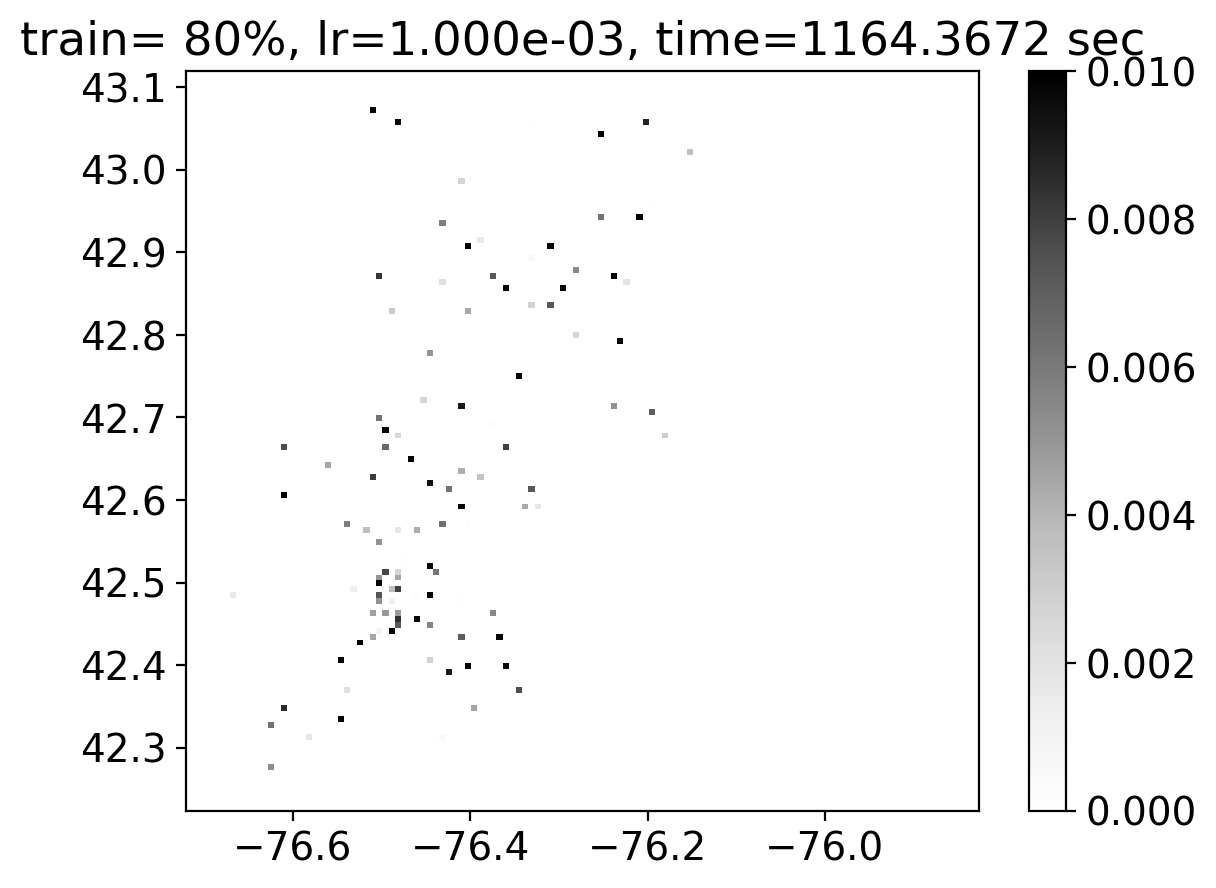
\includegraphics[width=\textwidth]{weights_map_plot_3}
        \caption[Predicted Probabilities of Agents Visiting Each Location Plotted on a Map (Latitude, Longitude) Representing Tompkins and Cortland Counties, NY]{Predicted Probabilities of Agents Visiting Each Location Plotted on a Map (Latitude, Longitude) Representing Tompkins and Cortland Counties, NY: Dark dots represent high prediction of visits. This can be compared to the plots for the 2-layered network and other models \cite[Figure 3]{Xue2016Avi2}.}
        \label{fig:Predicted Probabilities of Agents Visiting Each Location Plotted on a Map}
    \end{minipage}
\end{figure}

Observing that the average test loss values of learning rate = $10^{-3}$ is the lowest, we compare its results with the previous study's 2-layered network, historical data \cite[Table 1]{Xue2016Avi2}, and the 4-layered network with learning rate = $10^{-3}$ (see \Cref{sec:Identification Problem-Optimizing the Original Dataset}). As depicted in \Cref{fig:Comparison of Loss Values from Different Models of the Identification Problem}, our 3-layered neural network outperformed the previous 2-layered model by \textbf{0.14 units (14\% more closer to Ground Truth - $\matr{y}$)} \cite[Table 1]{Xue2016Avi2}, and also produced much better results (12\% more closer to Ground Truth) than the 4-layered model.

We also generated the predicted probabilities of the agents in the Test Set, visiting each location ($\matr{P}\matr{x}$), and plotted it onto maps marked by the locations' latitudes and longitudes. \Cref{fig:Predicted Probabilities of Agents Visiting Each Location Plotted on a Map} shows such a plot generated by the 3-layered network, where each dot represents a location.

To check if the model was overfitting at learning rate = $10^{-3}$, we plotted loss values at the end of each epoch for all tests. Although there remained $\approx$ 9\% difference (0.09 loss units) in the values of training and testing set, the 3-layered model was not drastically overfitting as an average \textit{end} difference of $8.76 \pm 1.59$\% persisted for many epochs, instead of increasing and tuning more to the training set. Even though one would expect overfitting with more tuned parameters, the 4-layered model also  produced an average \textit{end} difference of $16.77 \pm 4.73\%$, which persisted during the run. \Cref{fig:Train & Test Loss Values' Plots of Different Models} shows the results of a randomly selected experiment with plots of loss values at each epoch for the both networks.
\begin{figure}[!htbp]
    \centering
    \begin{subfigure}{.49\textwidth}
        \centering
        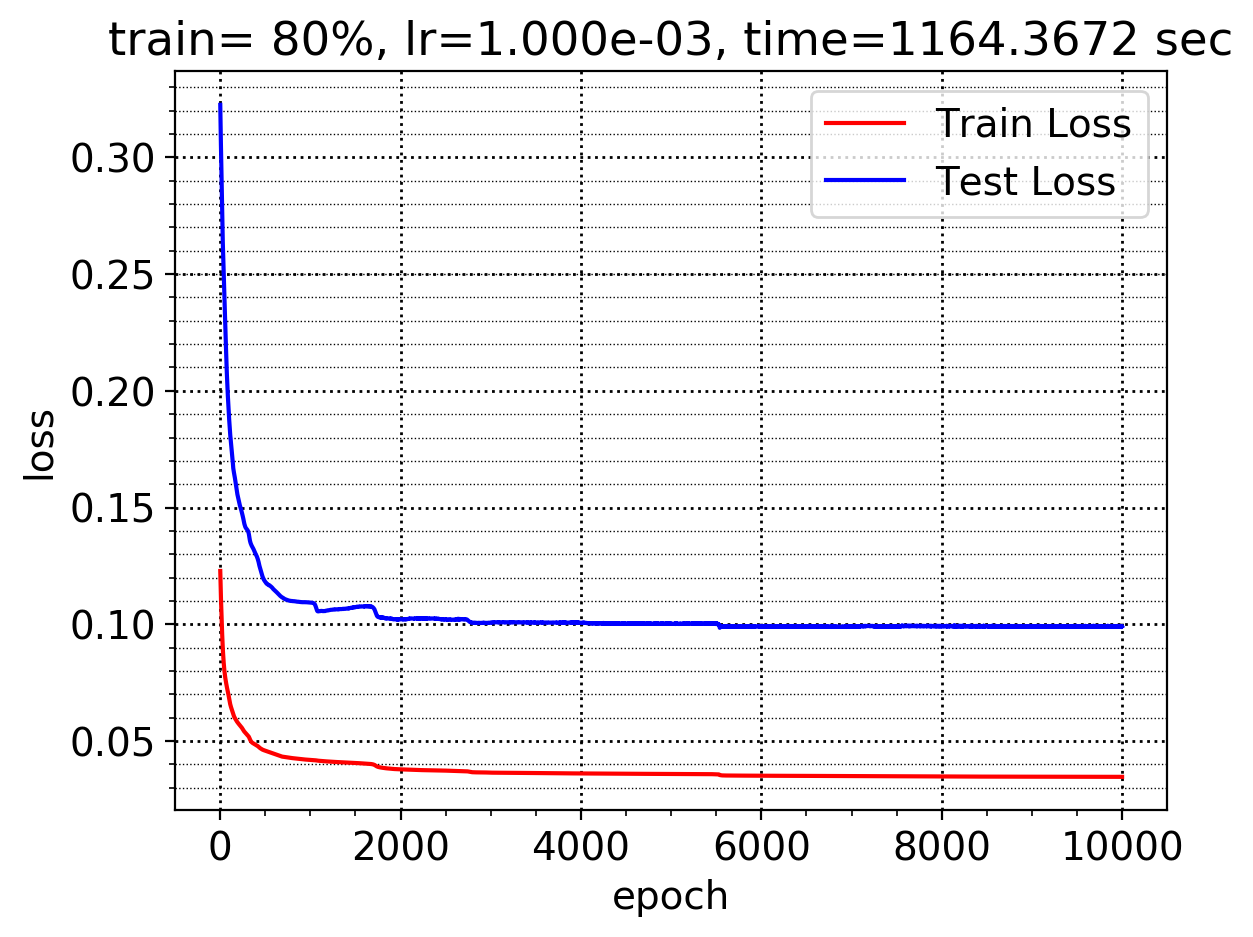
\includegraphics[width=\textwidth]{weights_train_test_loss_3_plot}
        \caption{Plot for 3-layered Model}
        \label{fig:Plot for 3-layered Model}
    \end{subfigure}
    \begin{subfigure}{.49\textwidth}
        \centering
        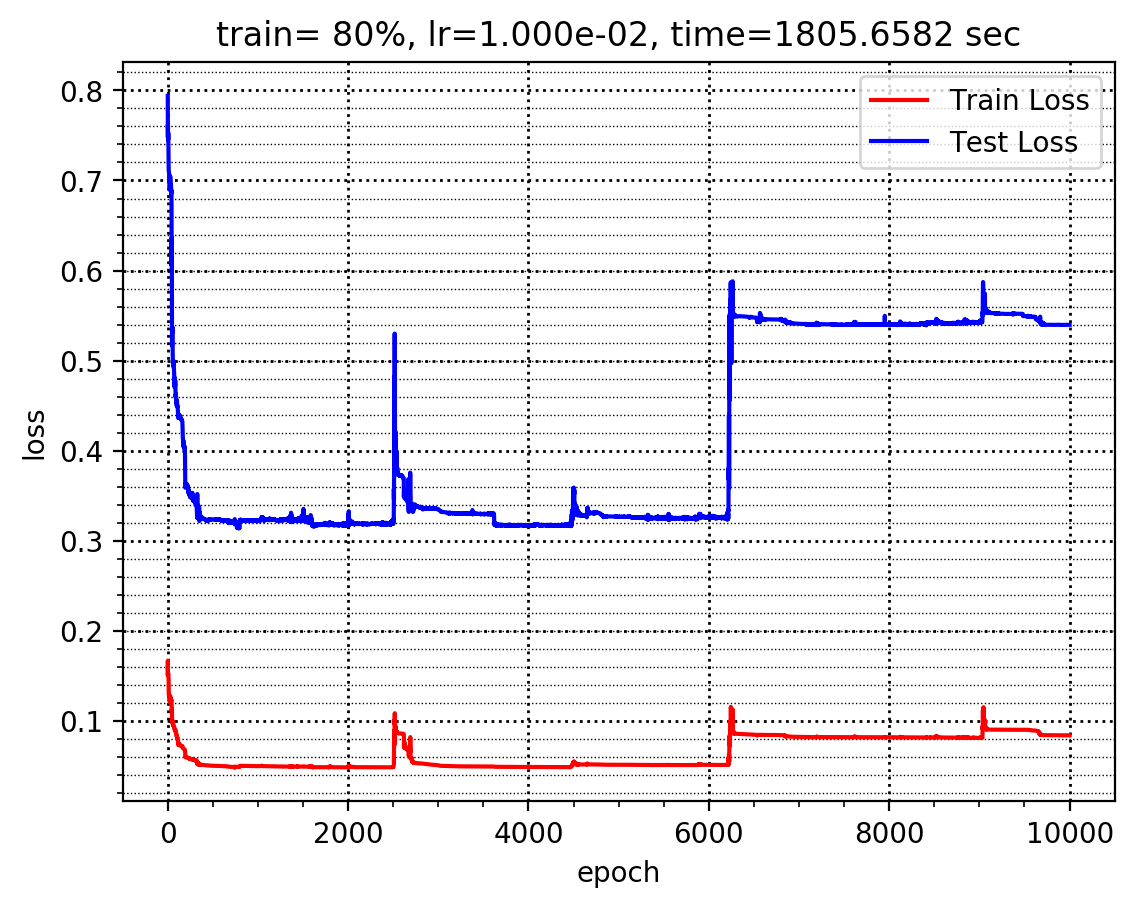
\includegraphics[width=\textwidth]{weights_train_test_loss_4_plot}
        \caption{Plot for 4-layered Model // todo}
        \label{fig:Plot for 4-layered Model}
    \end{subfigure}
    \caption[Train and Test Loss Values' Plots of Different Models]{Train and Test Loss Values' Plots of Different Models: Both networks learn the set of weights quickly, as displayed in the steep descent in loss values before $\approx$ 1000 epochs. This quick learning is due to the choice of \textsc{Gradient-Descent}($\cdot$) function - Adam's algorithm \cite{Adam}. Other algorithms like SGD \cite{SGD} and Adagrad \cite{Adagrad} learn relatively slowly.}
    \label{fig:Train & Test Loss Values' Plots of Different Models}
\end{figure}

\subsection{GPU Speedup Results} \label{sec:IdProbRes - GPU}
Running on batches of sizes $T = 17, 51, 85, 129, 173$ on a randomly generated dataset for 1000 epochs with both GPU and CPU ``set'' separately, we obtained information on full execution runtimes (both training and testing runtimes combined). The average results (over 3 different seeds for each batch) are plotted in \Cref{fig:Execution Times of Different Batch-Sizes with GPU and CPU ``set'' Separately}, which show promising GPU Speedup over CPU figures for any batch size; the GPU Speedup averaged over all tested batch-sizes is $\textbf{9.06}\pm\textbf{0.45}$.
\begin{figure}[!htbp]
    \centering
    \begin{subfigure}{.59\textwidth}
        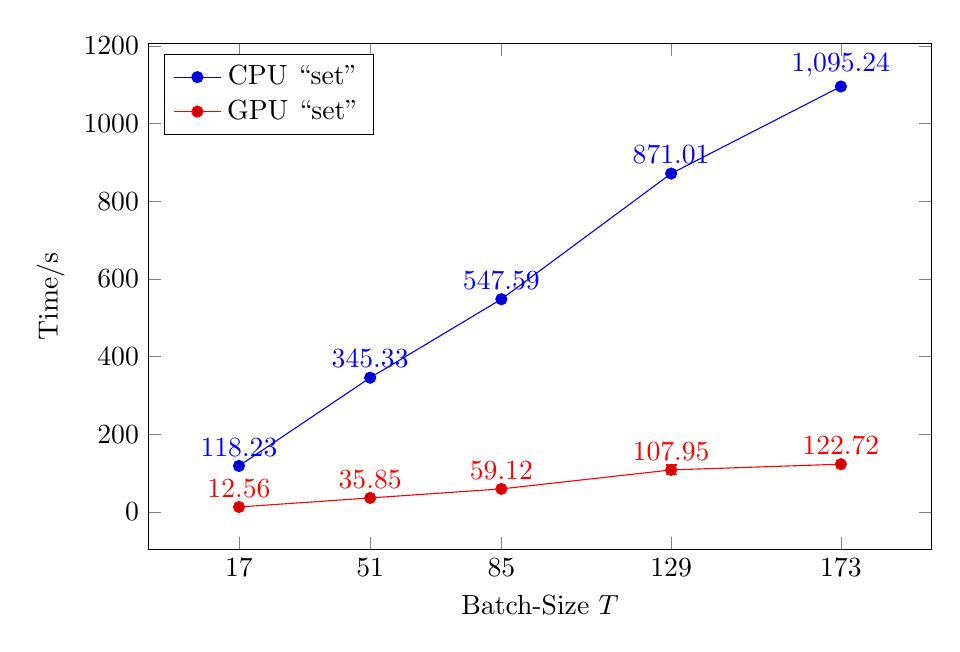
\begin{tikzpicture}
        \begin{axis}[
        width=.95\textwidth,
        height=8cm,
        xtick=data,
        xlabel={Batch-Size $T$},
        ylabel={Time/s},
        enlarge x limits=0.15,
        y tick label style={/pgf/number format/1000 sep=},
        extra y tick style={grid=major, tick label style={xshift=-1cm}},
        legend style={at={(0.02,.98)},
            anchor=north west},
        nodes near coords,
        ]
        \addplot+ [mark=*,error bars/.cd, y dir=both,y explicit] coordinates {
            (17,118.23) +- (1.77, 1.77)
            (51,345.33) +- (2.00, 2.00)
            (85,547.59) +- (1.76, 1.76)
            (129,871.01) +- (3.01, 3.01)
            (173,1095.24) +- (1.71, 1.71)
        };  % cpu
        \addplot+ [mark=*,error bars/.cd, y dir=both,y explicit] coordinates {
            (17,12.56) +- (0.022, 0.022)
            (51,35.85) +- (0.232, 0.232)
            (85,59.12) +- (0.131, 0.131)
            (129,107.95) +- (12.788, 12.788)
            (173,122.72) +- (0.169, 0.169)
        };  % gpu
        \legend{CPU ``set'',GPU ``set''}
        \end{axis}
        \end{tikzpicture}
    \end{subfigure}
    \begin{subfigure}{.4\textwidth}
        \centering
        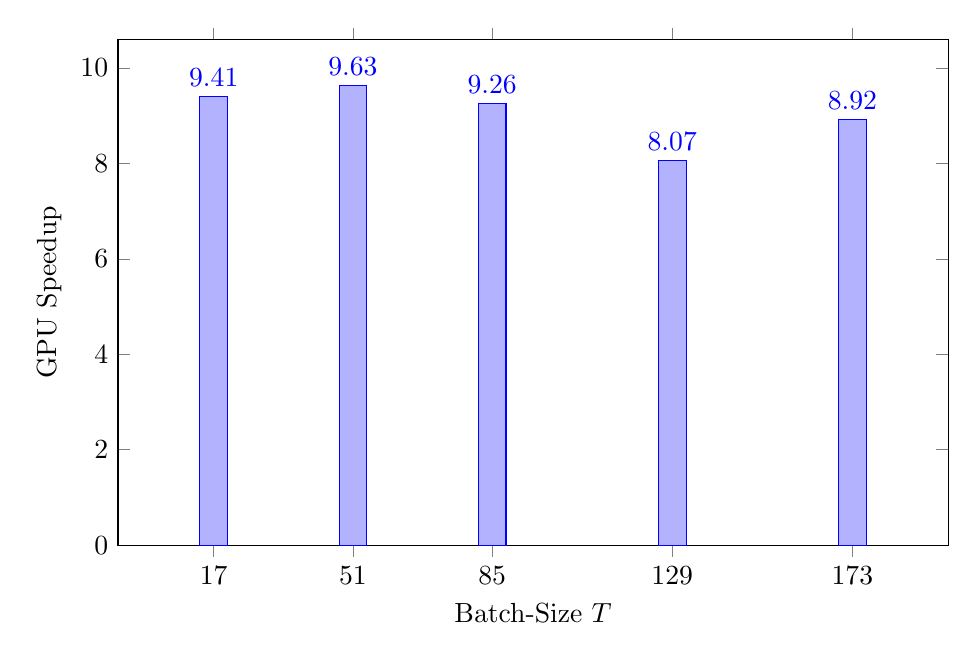
\begin{tikzpicture}
            \begin{axis}[
            ybar,
            width=\textwidth,
            height=8cm,
            xtick=data,
            xlabel={Batch-Size $T$},
            ylabel={GPU Speedup},
            ymin=0,
            enlarge x limits=0.15,
            extra y tick style={grid=major, tick label style={xshift=-1cm}},
            nodes near coords,
            ]
            \addplot+ coordinates {
                (17,9.41)
                (51,9.63)
                (85,9.26)
                (129,8.07)
                (173,8.92)
            };
            \legend{}
            \end{axis}
        \end{tikzpicture}
    \end{subfigure}
    \caption[Finding Weights - Execution Times of Different Batch-Sizes $T$ with GPU and CPU ``set'' Separately]{Finding Weights - Execution Times of Different Batch-Sizes $T$ with GPU and CPU ``set'' Separately: The GPU delivers faster computation than CPU even as the datasets' sizes grow - the average speedup is $9.06\pm0.45$. Also, the error bars are indiscernible because they are too small ($< 1\%$)}.
    \label{fig:Execution Times of Different Batch-Sizes with GPU and CPU ``set'' Separately}
\end{figure}

\section{Pricing Problem's Results} \label{sec:Pricing Problem's Results}
\subsection{Optimization Results} \label{sec:PriProbRes - Optimization}
Taking the approach mentioned in \Cref{sec:Pricing Problem-Optimizing the Original Dataset}, we obtained consistent loss values for each set of weights (even with differently seeded rewards). The best performing set of weights was set-2, using which the average loss value for the Pricing Problem hovered around $0.0079\%$. Next, running differently seeded rewards with different learning rates on set-2 of weights, we obtained the lowest loss value of $\textbf{0.0069\%}$.
%    \begin{figure}[!htbp]
%        \centering
%        \begin{tikzpicture}
%        \begin{axis}[
%        ybar,
%        width=.6\textwidth,
%        height=7cm,
%        enlarge x limits=0.15,
%        ylabel={Loss Value (in\%)},
%        symbolic x coords={Set-1,Set-2,Set-3,Set-4,Set-5},
%        xtick=data,
%        nodes near coords,
%        nodes near coords align={vertical},
%        xlabel={Models},
%        xlabel style={yshift=-.5cm}
%        ]
%        \addplot+ [error bars/.cd, y dir=both, y explicit] coordinates {
%            (Set-1, 0.0152) +- (0.0001, 0.0001)
%            (Set-2, 0.0079) +- (0.0005, 0.0005)
%            (Set-3, 0.0139) +- (0.0003, 0.0003)
%            (Set-4, 0.0129) +- (0.0002, 0.0002)
%            (Set-5, 0.0155) +- (0.0002, 0.0002)
%        };
%        \end{axis}
%        \end{tikzpicture}
%    \end{figure}

Compared to the proportional reward distribution (loss values calculated using set-2 of weights), our model's set of rewards produced loss value $\approx$ \textbf{3 times} lower. We again clarify that we compare the best loss values, as the organizer expects to find a distribution that is as optimal as possible.  \Cref{tab:Loss Values Calculated from Different Sets of Rewards} lists the best loss values obtained on each type of reward allocation (model's predicted, random and proportional - \Cref{sec:Pricing Problem-Optimizing the Original Dataset}).
\begin{table}[!htbp]
    \centering
    \caption[Loss Values Calculated from Different Sets of Rewards]{Loss Values Calculated from Different Sets of Rewards: The values are small because the loss function $Z_P(\vect{r})$ (\Cref{eqn:pricing_problem}) is averaged over the number of locations}
    \label{tab:Loss Values Calculated from Different Sets of Rewards}
    \begin{tabular}{|c|c|}
        \hline
        \textbf{Rewards Obtained From} & \textbf{Best Loss Values (In \%)}\\
        \hline
        Model's Prediction & 0.0069\\
        Random Initialization & 0.0331\\
        Proportional Distribution & 0.0235\\
        \hline
    \end{tabular}
\end{table}

\subsection{GPU Speedup Results} \label{sec:PriProbRes - GPU}
After running on different batch-sizes $J = 11, 35, 55, 85, 116, 145, 174, 203, 232$, we \textbf{did not observe drastic GPU speedup} for the full model. \Cref{fig:Finding Rewards - Time Taken by the Full Model} shows the Speedup trend: GPU Speedup for the full model was a mere \textbf{1.53 $\pm$ 0.10}.
\begin{figure}[!htbp]
    \centering
    \begin{subfigure}{\textwidth}
        \centering
        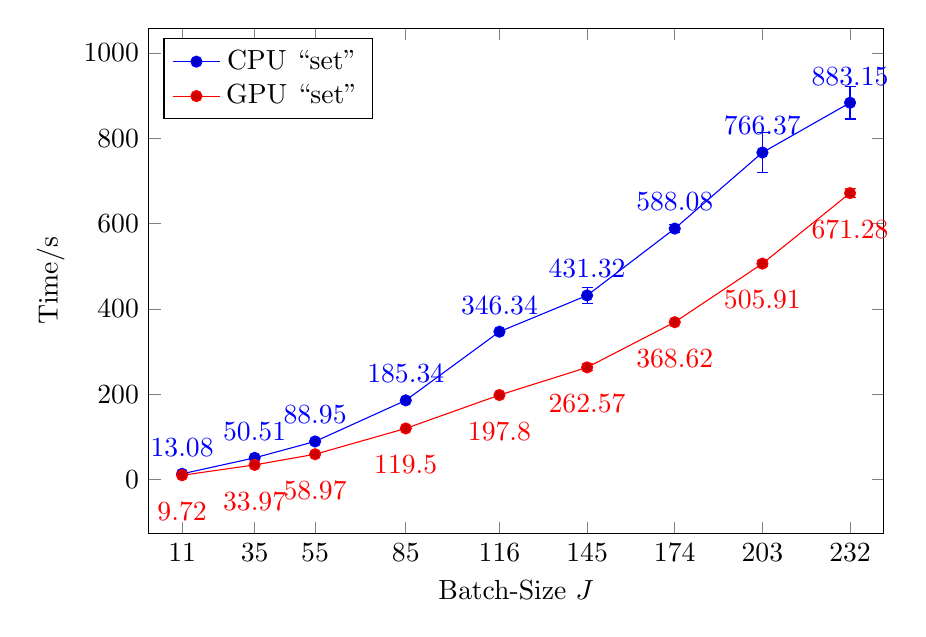
\begin{tikzpicture}
            \begin{axis}[
            width=.9\textwidth,
            height=8cm,
            xtick=data,
            xlabel={Batch-Size $J$},
            ylabel={Time/s},
            enlarge y limits=0.15,
            enlarge x limits=0.05,
            y tick label style={/pgf/number format/1000 sep=},
            extra y tick style={grid=major, tick label style={xshift=-1cm}},
            legend style={at={(0.02,.98)},
                anchor=north west},
            nodes near coords,
            every node near coord/.append style={yshift=-0.7cm}
            ]
            \addplot+ [mark=*,
            nodes near coords=\raisebox{0.8cm}{\pgfmathprintnumber\pgfplotspointmeta},error bars/.cd, y dir=both,y explicit
            ] coordinates {
                (11,13.08) +- (1.04, 1.04)
                (35,50.51) +- (1.73, 1.73)
                (55,88.95) +- (0.35, 0.35)
                (85,185.34) +- (0.95, 0.95)
                (116,346.34) +- (1.67, 1.67)
                (145,431.32) +- (18.06,18.06)
                (174,588.08) +- (10.16,10.16)
                (203,766.37) +- (47.02,47.02)
                (232,883.15) +- (38.00,38.00)
            };  % cpu
            \addplot+ [mark=*,error bars/.cd, y dir=both,y explicit] coordinates {
                (11,9.72) +- (0.08, 0.08)
                (35,33.97) +- (0.26, 0.26)
                (55,58.97) +- (0.19, 0.19)
                (85,119.50) +- (0.35, 0.35)
                (116,197.80) +- (4.02, 4.02)
                (145,262.57) +- (8.04,8.04)
                (174,368.62) +- (1.06,1.06)
                (203,505.91) +- (6.38,6.38)
                (232,671.28) +- (10.74,10.74)
            };  % gpu
            \legend{CPU ``set'',GPU ``set''}
            \end{axis}
        \end{tikzpicture}
        \caption{Time Taken by the Full Model: GPU Speedup over all batch-sizes is only \textbf{1.53 $\pm$ 0.10}.}
        \label{fig:Finding Rewards - Time Taken by the Full Model}
    \end{subfigure}\vspace*{1em}
    \begin{subfigure}{\textwidth}
        \centering
        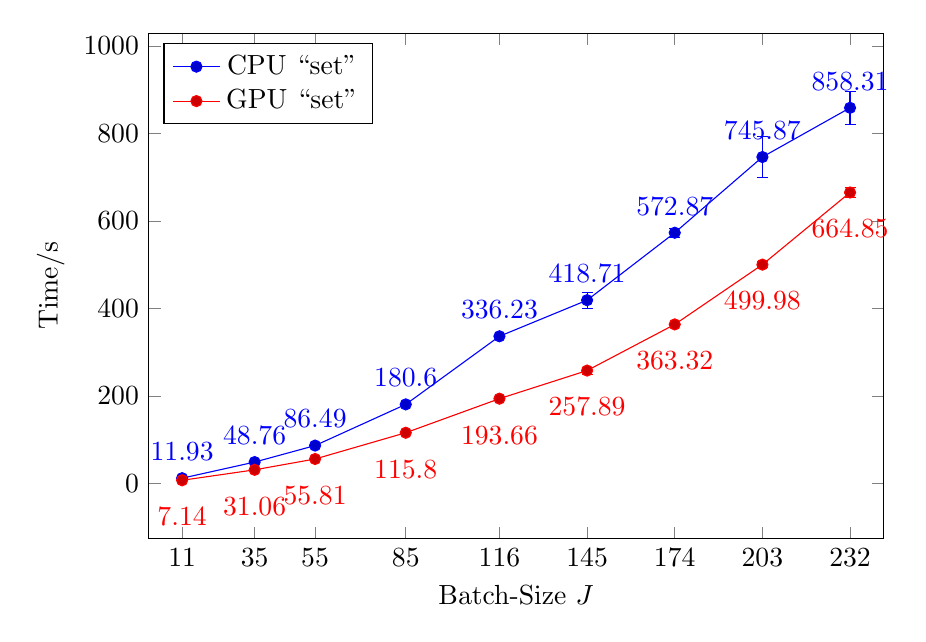
\begin{tikzpicture}
            \begin{axis}[
            width=.9\textwidth,
            height=8cm,
            xtick=data,
            enlarge y limits=0.15,
            enlarge x limits=0.05,
            xlabel={Batch-Size $J$},
            ylabel={Time/s},
            y tick label style={/pgf/number format/1000 sep=},
            legend style={at={(0.02,.98)},
                anchor=north west},
            nodes near coords,
            every node near coord/.append style={yshift=-0.7cm}
            ]
            \addplot+ [mark=*,
            nodes near coords=\raisebox{0.8cm}{\pgfmathprintnumber\pgfplotspointmeta},error bars/.cd, y dir=both,y explicit
            ] coordinates {
                (11,11.93) +- (0.94, 0.94)
                (35,48.76) +- (1.68, 1.68)
                (55,86.49) +- (0.36, 0.36)
                (85,180.60) +- (0.97, 0.97)
                (116,336.23) +- (1.46, 1.46)
                (145,418.71) +- (18.17,18.17)
                (174,572.87) +- (10.35,10.35)
                (203,745.87) +- (46.88,46.88)
                (232,858.31) +- (37.18,37.18)
            };  % cpu
            \addplot+ [mark=*,error bars/.cd, y dir=both,y explicit] coordinates {
                (11,7.14) +- (0.08, 0.08)
                (35,31.06) +- (0.26, 0.26)
                (55,55.81) +- (0.19, 0.19)
                (85,115.80) +- (0.35, 0.35)
                (116,193.66) +- (4.02, 4.02)
                (145,257.89) +- (8.01,8.01)
                (174,363.32) +- (1.03,1.03)
                (203,499.98) +- (6.37,6.37)
                (232,664.85) +- (10.73,10.73)
            };  % gpu
            \legend{CPU ``set'',GPU ``set''}
            \end{axis}
        \end{tikzpicture}
        \caption[Time taken by the LP]{Time taken by the LP: GPU Speedup over all batch-sizes is only \textbf{1.56 $\pm$ 0.08}. As discussed in \Cref{sec:PriProbRes - GPU,app:Strange GPU Speedup in LP Computation}, we shouldn't have witnessed this speedup as both configurations' LPs were computed on the CPU. Hence, we expected the GPU Speedup value for LP to be $\approx$ 1. }
        \label{fig:Finding Rewards - Time taken by the LP}
    \end{subfigure}
    \caption{Finding Rewards - Execution Times of Different Batch-Sizes $J$ with GPU and CPU ``set'' Separately}
    \label{fig:Finding Rewards - Execution Times of Different Batch-Sizes J with GPU and CPU ``set'' Separately}
\end{figure}

Since the the low GPU Speedup was uncanny, we looked for operations that were causing the program to slow down on the GPU. Since the 2-layered network was quite small, we suspected the LP problem (\Cref{eqn:lp_math_constrain_rewards,eqn:lp_code_constrain_rewards}) to influence the runtimes. Thus, we recorded execution times for both the neural network and the LP separately. As we suspected, the LP did impact the runtime more than the neural networks did, and accounted for $\approx 90 \%$ of the total model runtime (\Cref{fig:Finding Rewards - Execution Times of Different Batch-Sizes J with GPU and CPU ``set'' Separately}). However, the GPU Speedup in LP runtime was unusual.

\subsubsection{Strange GPU Speedup in LP Computation}
The Speedup is exceptional as we intentionally transferred the needed matrices/tensors to the CPU for solving the LP using Simplex. Since SciPy's Optimize Module uses a single CPU core and does not utilize the GPU, we expected similar runtimes for both configurations. Our efforts to determine the reasons are collected in \Cref{app:Strange GPU Speedup in LP Computation} instead of digressing here. As stated later in this section, we disregard the old GPU Speedup results for finding rewards and use the more suited ones.

We found that the LP in CPU ``set'' was slower than normal because of latency in thread synchronization\footnote{Pytorch uses OpenMP \cite{PTDocs,OpenMP} when the CPU is ``set'', which threads the 2-layered network.} (\Cref{app:Strange GPU Speedup in LP Computation}). Since \Cref{alg:Solving the Pricing Problem} performs operations sequentially (Calculate loss $\rightarrow$ Gradient-Descent and Update $\vect{r}$ $\rightarrow$ Constrain using LP), we suggest these possibilities:
\begin{enumerate}
    \item The 2-layered network is parallelized but \texttt{scipy.optimize}'s LP solver is not. Since both sub-problems are solved by independent frameworks, we could not thread the whole algorithm without implementing back-end OpenMP \cite{OpenMP} back-end manually and allowing multiple copies of the script to run simultaneously. Currently, the LP problem acts as a shared resource, requiring all network threads to synchronize before processing, causing time lag before all elements/matrices are available.
    \item The simultaneously running threads downgrade the LP solver's performance. We do not endorse this possibility because the CPU resources are independent when using multi-processing over CPU's cores. We checked if the same script running simultaneously on another core hampered the performance of the original copy, but did not witness any dependence.
\end{enumerate}

We believe the first possibility to be the reason (elaborated in \Cref{app:GPU Speedup in LP Computation}). While one might contend the lack of this behavior in GPU ``set'' even though it needs thread synchronization before starting the LP solver, we reiterate that we intentionally transfer the matrices to the CPU after the network has been executed, adding the time elapsed in the network's time logs. This is not case with CPU ``set'' because the network remains in execution in other cores while the LP has started. Therefore, when we restrict the script's access to a single CPU core, we do not witness any GPU Speedup in LP runtime. This only affects CPU ``set'' performance because the GPU ``set'' configuration independently executes the network on the GPU.
\begin{figure}[!htbp]
    \centering
    \begin{subfigure}{\textwidth}
        \centering
        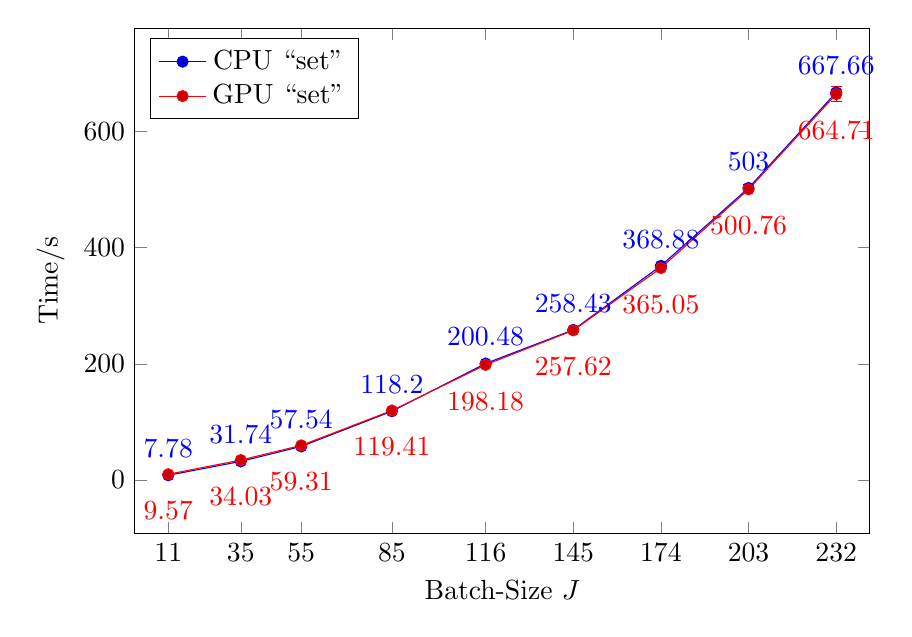
\begin{tikzpicture}
        \begin{axis}[
        width=.9\textwidth,
        height=8cm,
        xtick=data,
        xlabel={Batch-Size $J$},
        ylabel={Time/s},
        enlarge y limits=0.15,
        enlarge x limits=0.05,
        y tick label style={/pgf/number format/1000 sep=},
        extra y tick style={grid=major, tick label style={xshift=-1cm}},
        legend style={at={(0.02,.98)},
            anchor=north west},
        nodes near coords,
        every node near coord/.append style={yshift=-0.7cm}
        ]
        \addplot+ [mark=*,
        nodes near coords=\raisebox{0.8cm}{\pgfmathprintnumber\pgfplotspointmeta},error bars/.cd, y dir=both,y explicit
        ] coordinates {
            (11,7.78) +- (0.03,0.03)
            (35,31.74) +- (0.32,0.32)
            (55,57.54) +- (0.14,0.14)
            (85,118.20) +- (0.52,0.52)
            (116,200.48) +- (0.78,0.78)
            (145,258.43) +- (2.67,2.67)
            (174,368.88) +- (1.71,1.71)
            (203,503.00) +- (6.22,6.22)
            (232,667.66) +- (5.78,5.78)
        };  % cpu
        \addplot+ [mark=*,error bars/.cd, y dir=both,y explicit] coordinates {
            (11,9.57) +- (0.03,0.03)
            (35,34.03) +- (0.31,0.31)
            (55,59.31) +- (0.14,0.14)
            (85,119.41) +- (0.47,0.47)
            (116,198.18) +- (2.04,2.04)
            (145,257.62) +- (2.68,2.68)
            (174,365.05) +- (3.55,3.55)
            (203,500.76) +- (3.22,3.22)
            (232,664.71) +- (13.16,13.16)
        };  % gpu
        \legend{CPU ``set'',GPU ``set''}
        \end{axis}
        \end{tikzpicture}
        \caption{Time Taken by the Full Model: GPU Speedup over all batch-sizes is only $\textbf{0.97}\pm\textbf{0.04}$ - heavily impacted by LP runtimes.}
        \label{fig:Restricted Finding Rewards - Time Taken by the Full Model}
    \end{subfigure}\vspace*{1em}
    \begin{subfigure}{\textwidth}
        \centering
        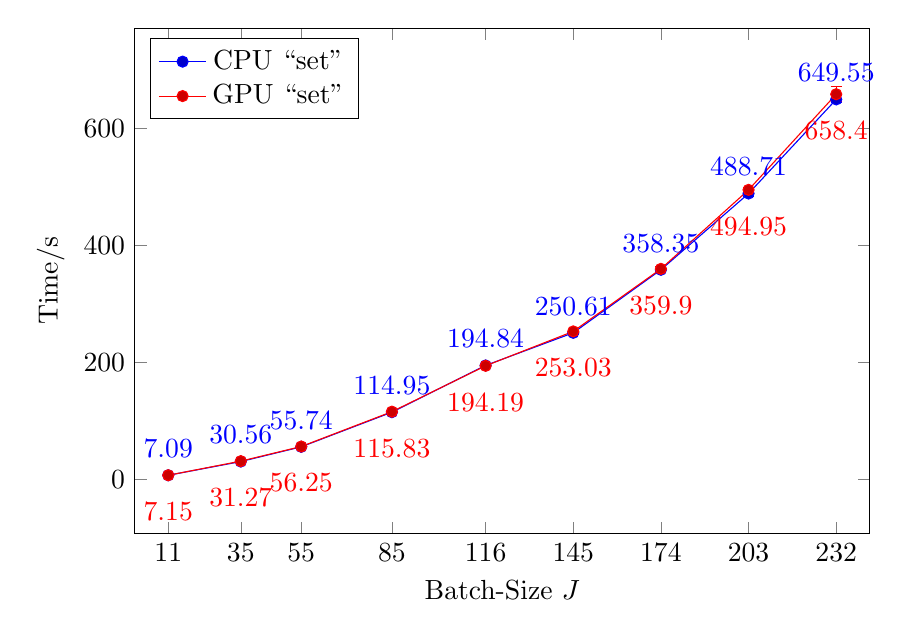
\begin{tikzpicture}
        \begin{axis}[
        width=.9\textwidth,
        height=8cm,
        xtick=data,
        enlarge y limits=0.15,
        enlarge x limits=0.05,
        xlabel={Batch-Size $J$},
        ylabel={Time/s},
        y tick label style={/pgf/number format/1000 sep=},
        legend style={at={(0.02,.98)},
            anchor=north west},
        nodes near coords,
        every node near coord/.append style={yshift=-0.7cm}
        ]
        \addplot+ [mark=*,
        nodes near coords=\raisebox{0.8cm}{\pgfmathprintnumber\pgfplotspointmeta},error bars/.cd, y dir=both,y explicit
        ] coordinates {
            (11,7.09) +- (0.04,0.04)
            (35,30.56) +- (0.32,0.32)
            (55,55.74) +- (0.14,0.14)
            (85,114.95) +- (0.49,0.49)
            (116,194.84) +- (0.84,0.84)
            (145,250.61) +- (2.47,2.47)
            (174,358.35) +- (1.68,1.68)
            (203,488.71) +- (5.74,5.74)
            (232,649.55) +- (5.93,5.93)
        };  % cpu
        \addplot+ [mark=*,error bars/.cd, y dir=both,y explicit] coordinates {
            (11,7.15) +- (0.04,0.04)
            (35,31.27) +- (0.30,0.30)
            (55,56.25) +- (0.13,0.13)
            (85,115.83) +- (0.47,0.47)
            (116,194.19) +- (2.03,2.03)
            (145,253.03) +- (2.67,2.67)
            (174,359.90) +- (3.57,3.57)
            (203,494.95) +- (3.20,3.20)
            (232,658.40) +- (13.15,13.15)
        };  % gpu
        \legend{CPU ``set'',GPU ``set''}
        \end{axis}
        \end{tikzpicture}
        \caption[Time taken by the LP]{Time taken by the LP: GPU Speedup over all batch-sizes is only $\textbf{0.99}\pm\textbf{0.005}$. Expectedly, there is no GPU Speedup in LP runtimes.}
        \label{fig:Restricted Finding Rewards - Time taken by the LP}
    \end{subfigure}
\end{figure}

\begin{figure}[!htbp]
    \centering
    \ContinuedFloat
    \begin{subfigure}{\textwidth}
        \centering
        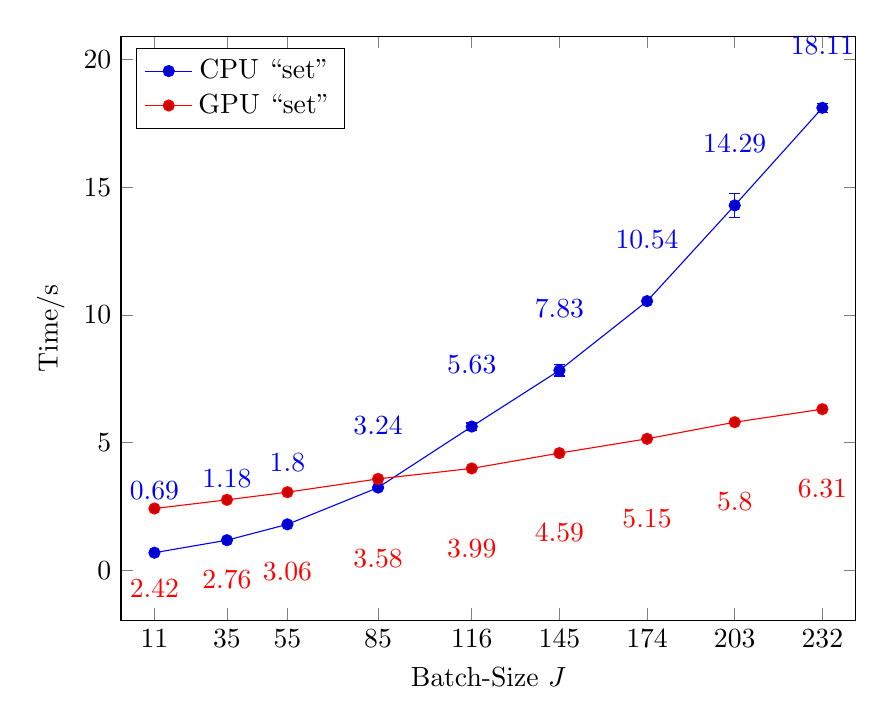
\begin{tikzpicture}
        \begin{axis}[
        width=.9\textwidth,
        height=9cm,
        xtick=data,
        enlarge y limits=0.15,
        enlarge x limits=0.05,
        xlabel={Batch-Size $J$},
        ylabel={Time/s},
        legend style={at={(0.02,.98)},
            anchor=north west},
        nodes near coords,
        every node near coord/.append style={yshift=-1.25cm}
        ]
        \addplot+ [mark=*,
        nodes near coords=\raisebox{1.8cm}{\pgfmathprintnumber\pgfplotspointmeta},error bars/.cd, y dir=both,y explicit] coordinates {
            (11,0.69) +- (0.004,0.004)
            (35,1.18) +- (0.002,0.002)
            (55,1.80) +- (0.01,0.01)
            (85,3.24) +- (0.03,0.03)
            (116,5.63) +- (0.14,0.14)
            (145,7.83) +- (0.22,0.22)
            (174,10.54) +- (0.03,0.03)
            (203,14.29) +- (0.48,0.48)
            (232,18.11) +- (0.17,0.17)
        };  % cpu
        \addplot+ [mark=*, error bars/.cd, y dir=both,y explicit] coordinates {
            (11,2.42) +- (0.01,0.01)
            (35,2.76) +- (0.01,0.01)
            (55,3.06) +- (0.01, 0.01)
            (85,3.58) +- (0.01,0.01)
            (116,3.99) +- (0.01,0.01)
            (145,4.59) +- (0.01,0.01)
            (174,5.15) +- (0.02,0.02)
            (203,5.80) +- (0.02,0.02)
            (232,6.31) +- (0.005,0.005)
        };  % gpu
        \legend{CPU ``set'',GPU ``set''}
        \end{axis}
        \end{tikzpicture}
        \caption{Time taken by the Neural Network: GPU Speedup over all batch-sizes is $\textbf{1.41}\pm\textbf{0.76}$ - as transfer time between RAM and GPU's internal memory dominates for smaller datasets. However, as batch-size increases, computation time dominates over transfer time - GPU ``set'' performs better than CPU ``set''.}
        \label{fig:Restricted Finding Rewards - Time taken by the Neural Network}
    \end{subfigure}\vspace*{1em}
    \begin{subfigure}{0.3\textwidth}
        \centering
        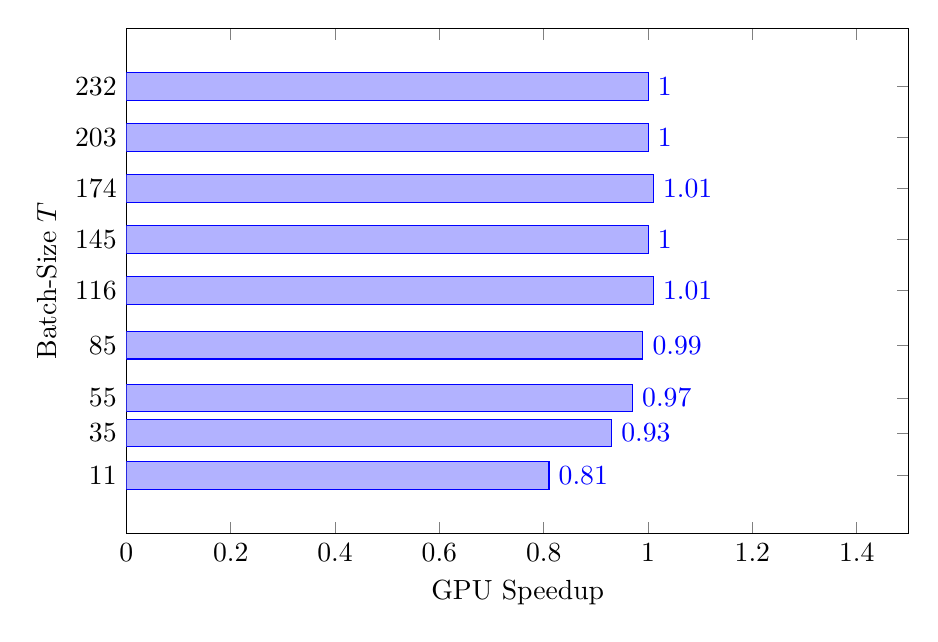
\begin{tikzpicture}
        \begin{axis}[
        xbar,
        width=0.95\textwidth,
        height=8cm,
        ytick=data,
        ylabel={Batch-Size $T$},
        xlabel={GPU Speedup},
        ytick align=inside,
        xmin=0,
        xmax=1.5,
        enlarge y limits=0.15,
        nodes near coords,
        ]
        \addplot+ coordinates {
            (0.81,11)
            (0.93,35)
            (0.97,55)
            (0.99,85)
            (1.01,116)
            (1.00,145)
            (1.01,174)
            (1.00,203)
            (1.00,232)
        };
        \end{axis}
        \end{tikzpicture}
        \caption{Speedup for the Full Model}
        \label{fig:Restricted Finding Rewards - Speedup for the Full Model}
    \end{subfigure}\hfill
    \begin{subfigure}{0.3\textwidth}
        \centering
        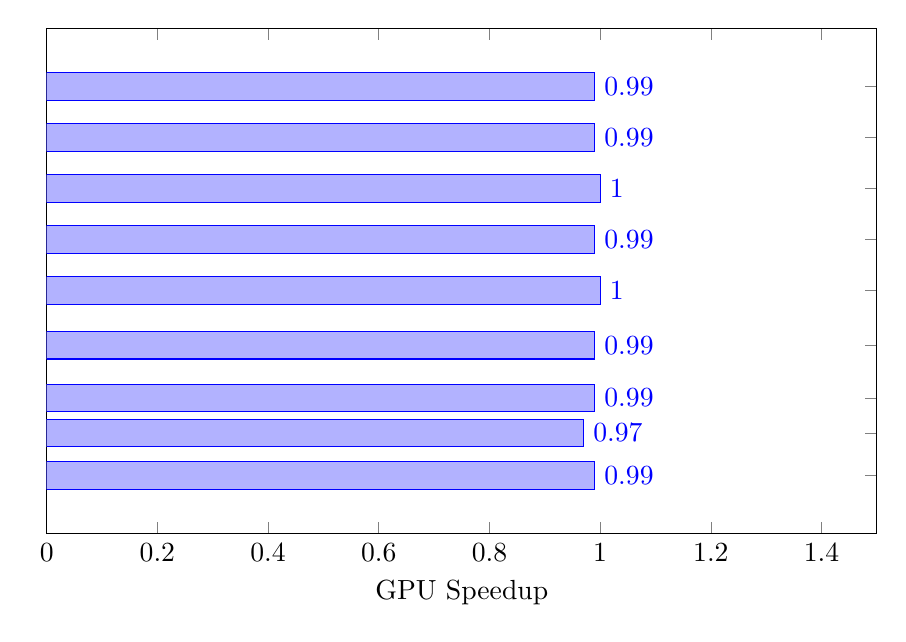
\begin{tikzpicture}
        \begin{axis}[
        xbar,
        width=\textwidth,
        height=8cm,
        ytick=data,
        yticklabels={,,},
        xlabel={GPU Speedup},
        ytick align=inside,
        xmin=0,
        xmax=1.5,
        enlarge y limits=0.15,
        nodes near coords,
        ]
        \addplot+ coordinates {
            (0.99,11)
            (0.97,35)
            (0.99,55)
            (0.99,85)
            (1.00,116)
            (0.99,145)
            (1.00,174)
            (0.99,203)
            (0.99,232)
        };
        \end{axis}
        \end{tikzpicture}
        \caption{Speedup for LP}
        \label{fig:Restricted Finding Rewards - Speedup for LP}
    \end{subfigure}\hfill
    \begin{subfigure}{0.4\textwidth}
        \centering
        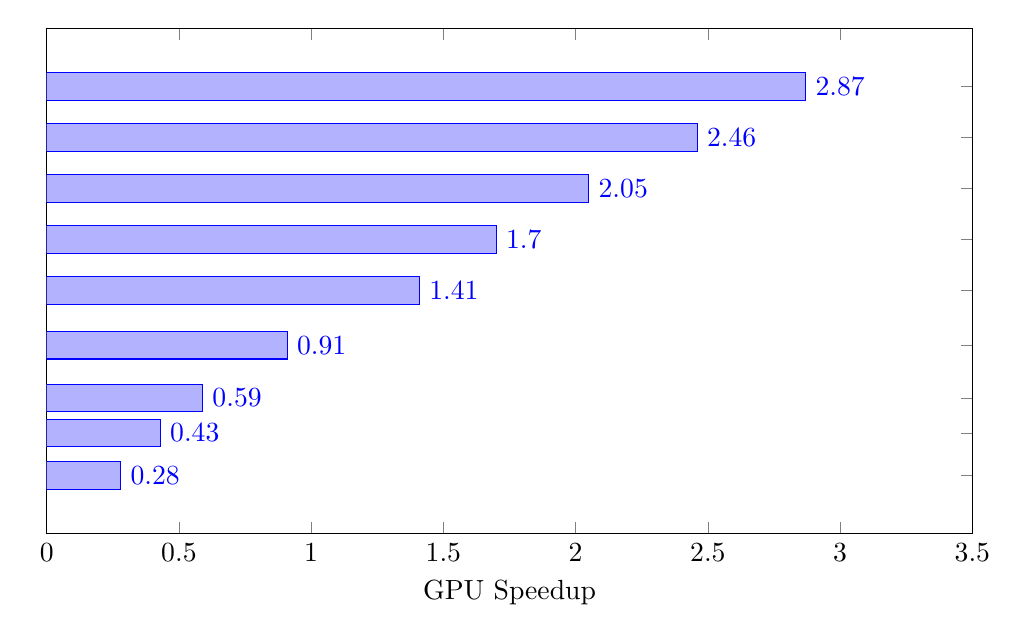
\begin{tikzpicture}
        \begin{axis}[
        xbar,
        width=1.1\textwidth,
        height=8cm,
        ytick=data,
        yticklabels={,,},
        xlabel={GPU Speedup},
        ytick align=inside,
        xmin=0,
        xmax=3.5,
        enlarge y limits=0.15,
        nodes near coords,
        ]
        \addplot+ coordinates {
            (0.28,11)
            (0.43,35)
            (0.59,55)
            (0.91,85)
            (1.41,116)
            (1.70,145)
            (2.05,174)
            (2.46,203)
            (2.87,232)
        };
        \end{axis}
        \end{tikzpicture}
        \caption{Speedup for the Neural Network}
        \label{fig:Restricted Finding Rewards - Speedup for the Neural Network}
    \end{subfigure}
    \caption[Finding Rewards After Restricing Script's Access to CPU Cores - Execution Times of Different Batch-Sizes $J$ with GPU and CPU ``set'' Separately]{Finding Rewards After Restricing Script's Access to CPU Cores - Execution Times of Different Batch-Sizes $J$ with GPU and CPU ``set'' Separately: Scaling is strongly hampered by the LP solver. Comparing the contributions of LP and Neural Network to total runtime on GPU ``set'', LP accounts for $\textbf{94.57}\pm\textbf{5.01}\%$ of the total time.}
    \label{fig:Restricted Finding Rewards - Execution Times of Different Batch-Sizes J with GPU and CPUa ``set'' Separately}
\end{figure}

\subsubsection{Final Results}
The results after restricting script's access to a single CPU cores are plotted in \Cref{fig:Restricted Finding Rewards - Execution Times of Different Batch-Sizes J with GPU and CPUa ``set'' Separately}. We prefer using these results (over previous results - \Cref{fig:Finding Rewards - Execution Times of Different Batch-Sizes J with GPU and CPU ``set'' Separately}) after restricting access, as it gives the better performance for CPU ``set''. The time elapsed for the Neural Network includes time taken to transfer tensors to and from the GPU, which results in overhead - as seen in higher runtimes for smaller datasets (lower batch-size) in \Cref{fig:Restricted Finding Rewards - Time taken by the Neural Network,fig:Restricted Finding Rewards - Speedup for the Neural Network}. However, as the batch-size increases, we see the computation dominating over the transfer time, resulting in higher CPU ``set'' runtimes; the GPU ``set'' runtimes almost grow linearly for the tested batch-sizes.

Moreover, the LP subproblem highly impacts the full model, accounting for more than $90\%$ of the total runtime. Therefore, even though the Neural Network gets sped up at bigger datasets, the GPU Speedup is not reflected in the full model.